% add style folder to path
\makeatletter
\def\input@path{{../style/}}
\makeatother

\documentclass[t, aspectratio=169, english, table]{tudelft-beamer}

% theorem
\newtheoremstyle{customthm}
{}
{}
{\upshape}
{}
{\bfseries}
{.}
{.5em}
{}
\theoremstyle{customthm}
\newtheorem{theorem}{Theorem}[chapter]
\newtheorem{definition}{Definition}[chapter]


% pgf figures
\usepackage{pgf}
\usepackage{tikz}
\usepackage{tikz-cd}
\usepackage{pgfplots}
\pgfplotsset{compat=1.14}
% \usepackage{lmodern}
\usepackage{import}
\def\mathdefault#1{#1}
\everymath=\expandafter{\the\everymath\displaystyle}

% comment macros
\newif\ifshowcomments
\showcommentstrue
% \showcommentsfalse
\ifshowcomments
    \newcommand{\mynote}[2]{\fbox{\bfseries\sffamily\scriptsize{#1}}
        {\small$\blacktriangleright$\textsf{\emph{#2}}$\blacktriangleleft$}}
    \newcommand{\citehere}[0]{\textcolor{red}{\fbox{\bfseries\sffamily\scriptsize{CITATION}}}}
\else
    \newcommand{\mynote}[2]{}
    \newcommand{\citehere}[0]{}
\fi
\newcommand{\todo}[1]{\textcolor{blue}{\mynote{To do}{#1}}}

% subfiles (for chapters)
\usepackage{subfiles}

% subfile macros
\newcommand{\onlyinsubfile}[1]{#1}
\newcommand{\notinsubfile}[1]{}

% Bibliography
\usepackage[backend=biber, style=apa, citestyle=numeric-comp]{biblatex}

\addbibresource[type=file, glob, datatype=bibtex, location=local]{../bibliography.bib}

% redefine image path
\graphicspath{{../images}{../figures}}

% main title
\title[]{Sharpened CG Iteration Bound for High-contrast Heterogeneous Scalar Elliptic PDEs}
\subtitle{Going Beyond Condition Number}
\author[]{P.~Soliman\inst{1}}

% define a graphic to be shown next to the title
\titlegraphic{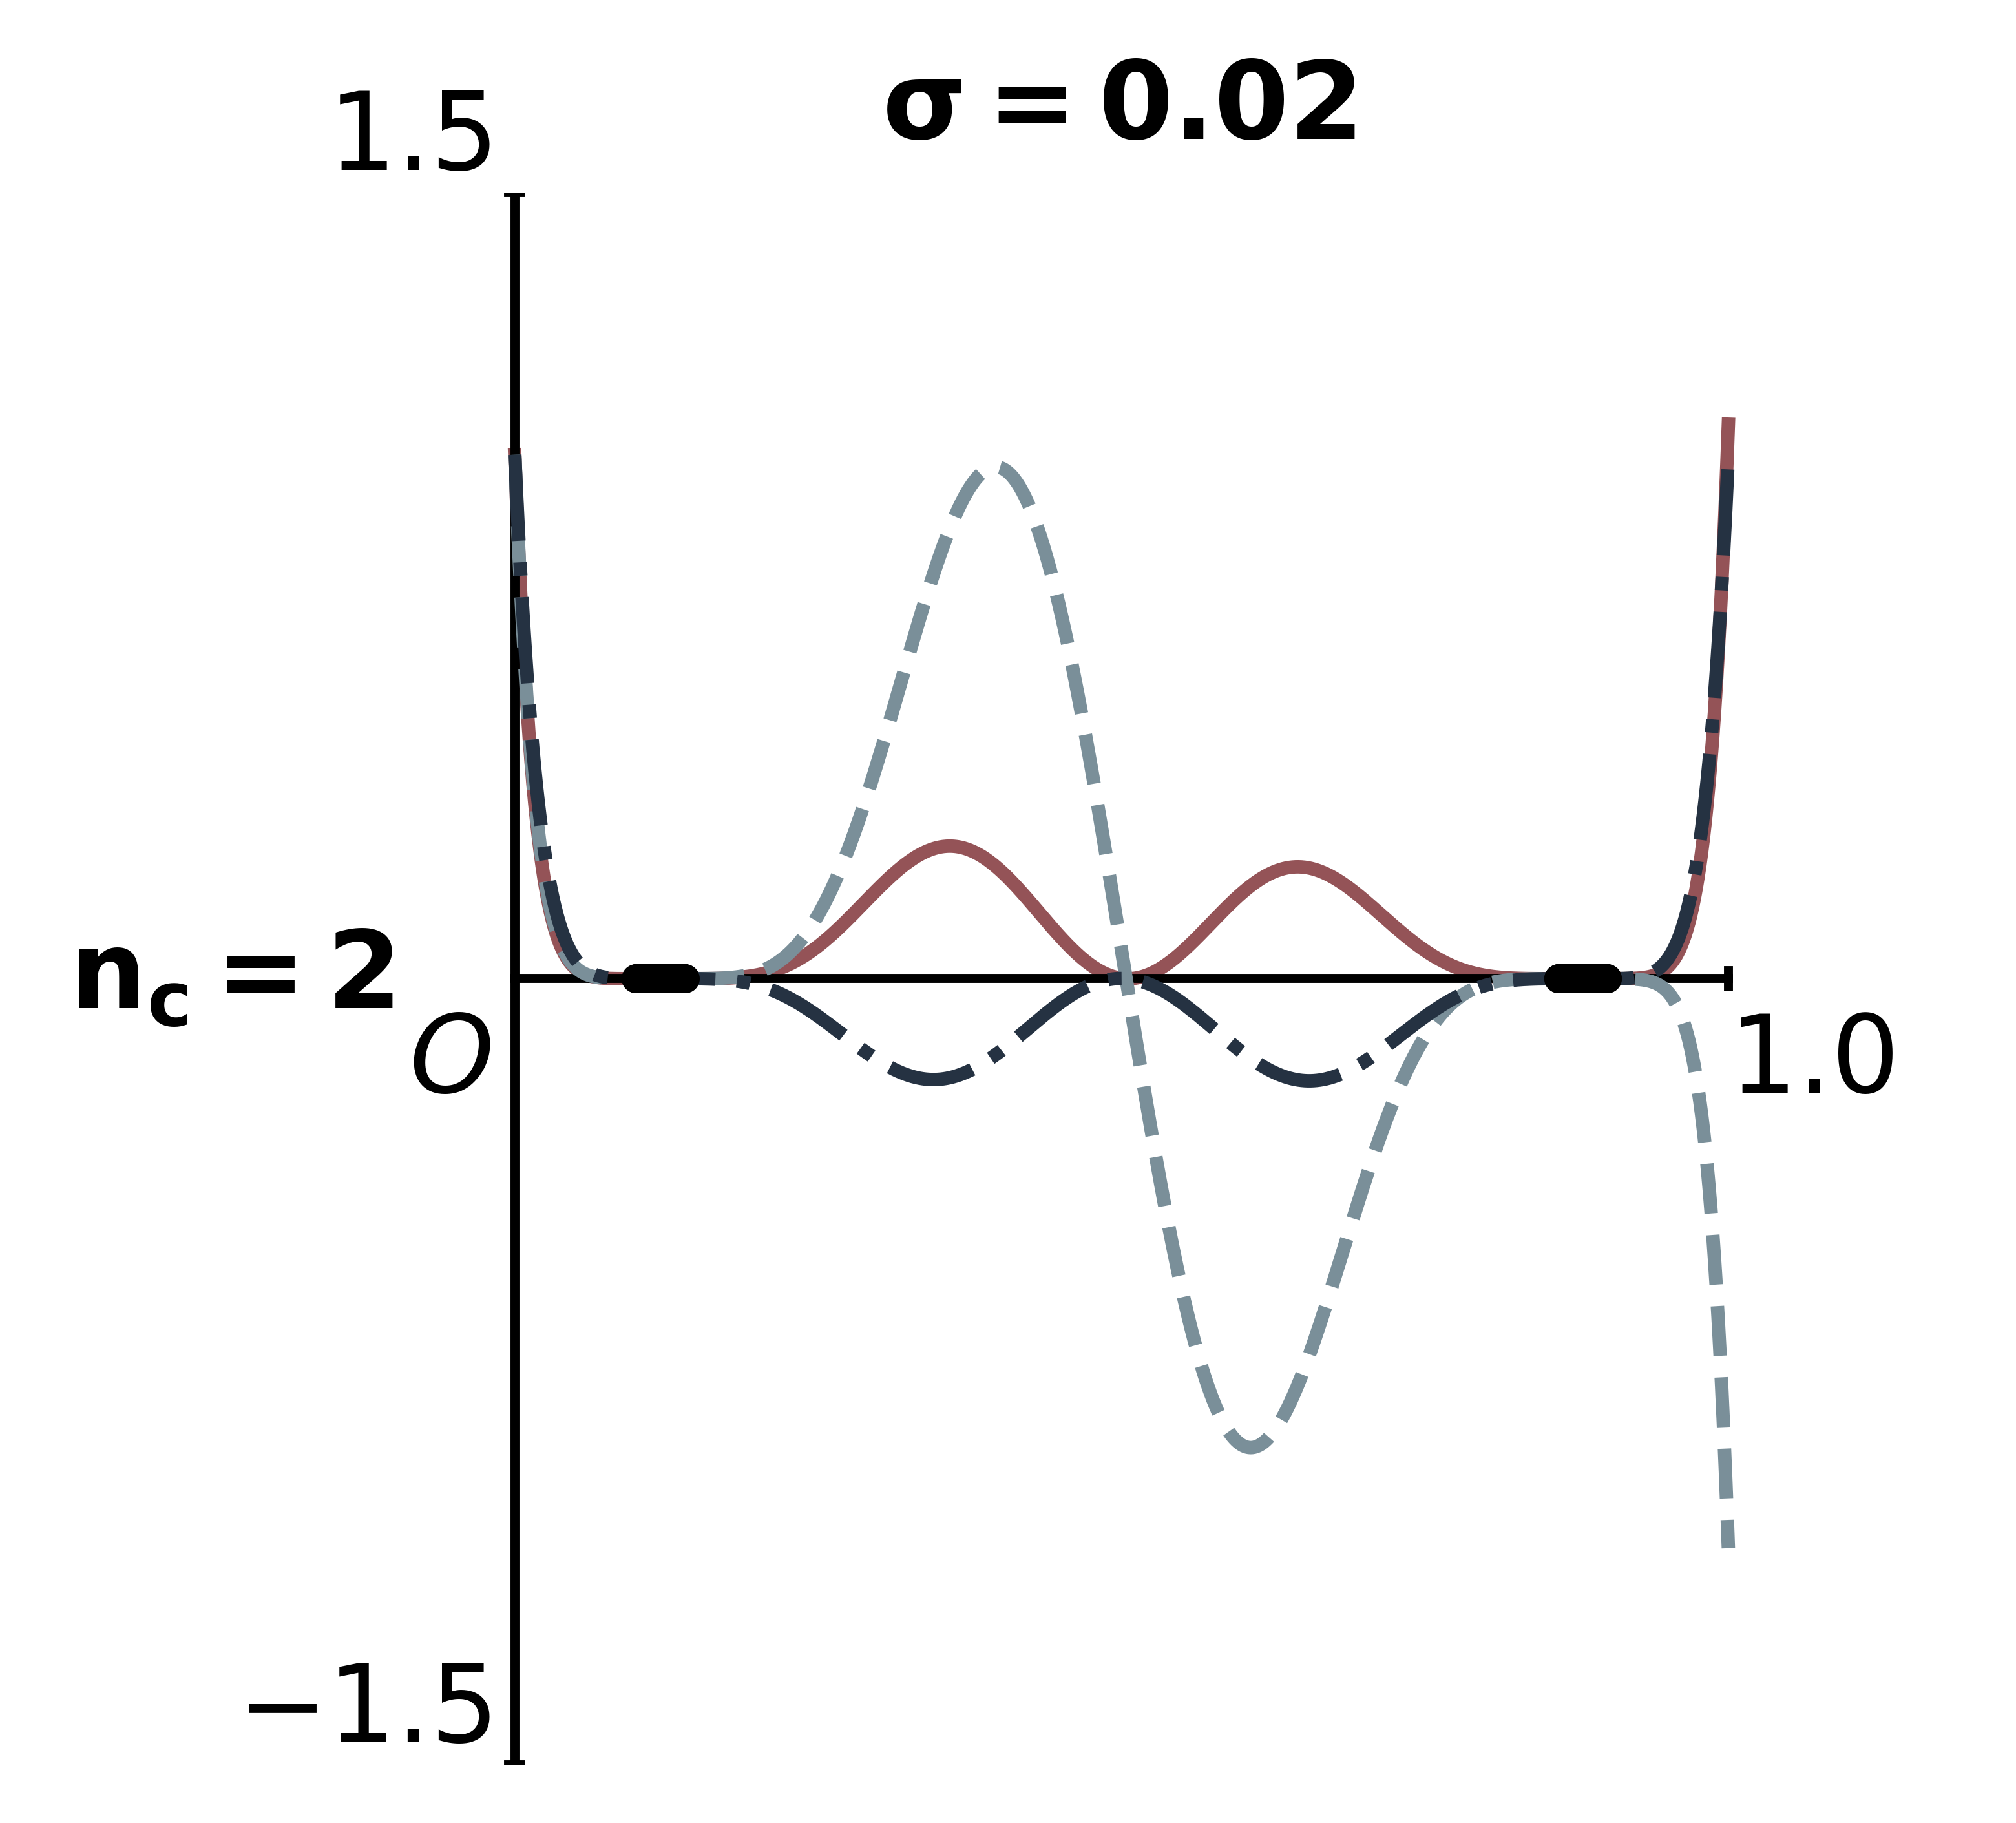
\includegraphics[width=0.4\paperwidth]{two_cluster_respoly.png}}

\institute[University]{
  \strut\llap{\inst{1}\,}Delft University of Technology
}
\date[EEMCS-DIAM-NA MSc. Thesis \monthyeardate]{EEMCS-DIAM Numerical Analysis MSc. Thesis Presentation, \monthyeardate}

% command for including images
\newcommand{\absimage}[4][0.5,0.5]{%
	\begin{textblock}{#3}%width
		[#1]% alignment anchor within image (centered by default)
		(#2)% position on the page (origin is top left)
		\includegraphics[width=#3\paperwidth]{#4}%
	\end{textblock}%
}

\begin{document}

\titleframe

\begin{frame}[label=opening]{Darcy Problem}
    \frametitle{Opening}
    \framesubtitle{Darcy Problem}
\end{frame}

\begin{frame}[label=opening]{Conjugate Gradient Method}
    \frametitle{Opening}
    \framesubtitle{Conjugate Gradient Method}
\end{frame}

\begin{frame}[label=opening]{Condition Number}
    \frametitle{Opening}
    \framesubtitle{Condition Number}
\end{frame}

\begin{frame}[label=opening]{Preconditioners}
    \frametitle{Opening}
    \framesubtitle{Preconditioners}
\end{frame}

\begin{frame}[label=opening]{Research Gap}
    \frametitle{Opening}
    \framesubtitle{Research Gap}
\end{frame}

\begin{frame}[label=toc]{Structure}
    \frametitle{Structure}
    \begin{itemize}
        \item Introducing CG
        \item How Does CG Converge? The Role of Eigenvalues
        \item Preconditioning: Taming High-Contrast Problems
        \item High-contrast coefficients: split eigenspectrum
        \item Towards Sharper Iteration Bounds
        \item Multi-Cluster Spectra
        \item How Sharp Are the New Bounds?
        \item New Bounds in Practice: Using Ritz Values
        \item Conclusion: Key Takeaways \& Future Directions
    \end{itemize}
\end{frame}

\begin{comment}
Level 0: Opening (no header)
- Opening question: "What do X, Y, Z have in common?". (Show X, Y and Z with single picture slides and make sure to give short descriptions. Go quickly through the single-picture slides.)
- Answer: "They can all be modelled by a..." high-contrast diffusion problem for $u, u_D \in H^1(\Omega)$, $f\in L^2(\Omega)$ and $\mathcal{C}\in L^{\infty}(\Omega)$
    \begin{equation*}
        \begin{aligned}
            -\nabla\cdot\left(\mathcal{C}\nabla u\right) & = f \quad \text{in } \Omega           \\
            u                                            & = u_D \quad \text{on } \partial\Omega
        \end{aligned}
    \end{equation*}
- Understanding the problem: We need to find $u \in H^1(\Omega)$ such that the above equation holds.
- Briefly explain why discretization is necessary for PDEs, for non-experts.
- Linear system of equations $A\mathbf{u}=\mathbf{b}$
- We can compute approximations $\mathbf{u}_1, \mathbf{u}_2, \ldots$ efficiently using the CG method.
- Main R.Q.: "How can improve existing estimates on the total number of necessary CG iterations?"
- FEM discretization $\Omega\rightarrow\mathcal{T}$, $\nabla \rightarrow A$, $u\rightarrow\mathbf{u}$, $f\rightarrow\mathbf{b}$

Level 1: Introducing CG
- CG takes in initial guess $\mathbf{u}_0$ and provides updated solution $\mathbf{u}_k$ after $k$ iterations.
- Classical bound given relative error tolerance $\epsilon_m = \frac{\|\mathbf{e}_m\|_A}{\|\mathbf{e}_0\|_A} \leq \epsilon$ is
$\epsilon_m \leq 2\left(\frac{\sqrt{\kappa} - 1}{\sqrt{\kappa} + 1}\right)^{m} \longrightarrow m \leq \left\lfloor\frac{\sqrt{\kappa}}{2}\ln\left(\frac{2}{\epsilon}\right) + 1\right\rfloor = m_1(\kappa)$
- However $m_1$ can be too pessimistic for high-contrast problems. That is, $m \ll m_1$
- Restate R.Q.: "How do we improve/sharpen the classical bound $m_1$ for model problem?"

Level 2: How Does CG Converge? The Role of Eigenvalues
- When discussing eigenvalues, a simple visual or analogy could help non-mathematicians.
- Spectrum $\sigma(A) = \{\lambda_1, \ldots, \lambda_n\}$ and $\kappa(A) = \frac{\lambda_{\max}}{\lambda_{\min}}$
- CG solution given as $\mathbf{u}_m = \mathbf{u}_0 + q(A)\mathbf{r}_0$, with polynomial $q$ being the \textit{solution polynomial}.
- CG residual polynomial $r(\lambda) = 1 - \lambda q(\lambda)$
- Error expression $\epsilon_m = \frac{\|\mathbf{e}_m\|_A}{\|\mathbf{e}_0\|_A} < \min_{r \in \mathcal{P}_{m-1}, r(0) = 1} \max_{\lambda \in \sigma(A)} |r(\lambda)|$
- Animation: cg_residual_poly
- Loop through different randomized, clustered spectra, showing r_m for each.
- Show best and worst case scenario's for CG convergence
- Restate R.Q.: "How can we construct an CG iteration bound that accounts for the influence of the eigenvalue distribution?"

Level 3: Preconditioning: Taming High-Contrast Problems
- Why do we want to account for eigenvalue distribution? (practical motivation)
- High-contrast $C$ leads to spectral gap and $\kappa(A)\gg1$
- Clarify what "preconditioning" means in practical terms (e.g., analogy to making a problem easier to solve).
- Mathematically: transform $A\mathbf{u}=\mathbf{b}$ into $M^{-1}A\mathbf{u}=M^{-1}\mathbf{b}$, with preconditioner $M$. This leads to a reduced spectral gap and lower conditioner number. Then, apply CG as usual (now called Preconditioned CG or PCG)
- Show Filipe & Alexander's Research: they used three kinds of preconditioners $M_1, M_2, M_3$ and all had similar conditioner numbers and thereby similar upper bounds for their iteration number, $m_1(\kappa)$.
- However, on a sample problem PCG with $M_1,M_2$ needed significantly less iterations than PCG with $M_3$.
- Restate R.Q.: "How can we construct a CG iteration bound that can distinguish between different preconditioners with similar conditioner numbers?"

Level 4: Towards Sharper Iteration Bounds
- Recap: $\epsilon_m < \min_{r \in \mathcal{P}_{m-1}, r(0) = 1} \max_{\lambda \in \sigma(A)} |r(\lambda)| \leq \epsilon$
- Head-on strategy for a bound: try to find an $m^{\text{th}}$-order polynomial that satisfies the min-max problem.
- Classical bound invokes: optimal Chebyshev polynomial $r(\lambda) = \hat{C}_m$, under the assumption of a uniform interval of eigenvalues $\sigma(A) = [\lambda_{\min}, \lambda_{\max}]$ (inaccurate!).
- Simplest non-trivial case (one spectral gap): two disjoint clusters
- Axelsson, assume two uniform intervals and invoke $r(\lambda) = \hat{C}_{p}\hat{C}_{p-m}$
- Resulting two-cluster bound $m_2(\kappa, \kappa_l, \kappa_r)=\left\lfloor\frac{\sqrt{\kappa_r}}{2} \ln (2 / \epsilon)+\left(1+\frac{\sqrt{\kappa_r}}{2} \ln \left(\frac{4\kappa}{\kappa_l}\right)\right) p\right\rfloor$
- Restate R.Q.: "How can we construct an CG iteration bound that accounts for the influence of the eigenvalue distribution for general spectra?"

Note: The transition from classical bounds to multi-cluster bounds could be made more explicit—perhaps with a summary slide or visual.

Level 5: Multi-Cluster Spectra
- Depending on coefficient function and preconditioned systems we can have any number of clusters.
- Extend Axelsson idea: $r(\lambda) = \hat{C}^{(1)}_{p_1}\hat{C}^{(2)}_{p_2}\ldots\hat{C}^{(k)}_{p_k} = \prod_{i=1}^{k} \hat{C}^{(i)}_{p_i}$
- Multi-cluster bound: $p_i \leq \left\lceil\log_{f_i}{\frac{\epsilon}{2}} + \sum_{j=1}^{i-1} p_j\log_{f_i}\left(\frac{\zeta^{(j)}_2}{\zeta^{(i,j)}_1}\right)\right\rceil$ and $m_{N_{\text{cluster}}} = \sum_{i=1}^{N_{\text{cluster}}} p_i$, depends on the extremal eigenvalues of \textit{each cluster}
- We need a way of partitioning a given spectrum $\sigma(A)$ into $N_{\text{cluster}}$ clusters.
- Idea: simple, we split at the largest (relative) gap between subsequent eigenvalues, check if the two resulting clusters would give a sharper bound than just one uniform cluster, that is $m_2(\kappa, \kappa_l, \kappa_r) < m_1(\kappa)$. If so, we split the clusters and repeat the process for each created cluster. If not, we stop partitioning. In the process we keep track of all the extremal eigenvalues. After partitioning, we calculate $m_{N_{\text{cluster}}}$.
- Animation: cluster_partitioning, visualize above partitioning and subsequent calculation $m_{N_{\text{cluster}}}$.
- Restate R.Q.: "How much sharper is $m_{N_{\text{cluster}}}$ compared to $m_1(\kappa)$ for our model problem?"

Level 6: How Sharp Are the New Bounds?
- We implement the model problem with the two coefficient functions that Filipe and Alexander used and solve them using PCG with preconditioners $M_1, M_2, M_3$.
- First experiment: For each $\sigma(M_i^{-1}A)$, we compute $m_{N_{\text{cluster}}}$ and $m_1(\kappa)$ for comparison. As well as, $m_{N_{\text{tail-cluster}}}$, a variant of $m_{N_{\text{cluster}}}$ that can take in clusters as well as individual eigenvalues.
- Results: the new bounds are incredibly sharp as they are anywhere from 2 to 4 times as big as $m$. For comparison, $m_1$ is anywhere from 100 to 1000 times bigger than $m$, where the difference increases for spectra with larger spectral gaps
- Restate R.Q.: "How can we compute $m_{N_{\text{cluster}}}$ for our model problem in practice?"

Level 7: New Bounds in Practice: Using Ritz Values
- Problem: computing $m_{N_{\text{cluster}}}$ requires a good estimate of $\sigma(M_i^{-1}A)$.
- Luckily, PCG gives us exactly that, every iteration it produces a set of so-called Ritz values that is `close' to the true eigenvalue distribution. In particular, at the $k^{\text{th}}$ iteration, we get a set of $k$ Ritz values that we can use as an approximation of the full spectrum $\sigma(M_i^{-1}A)$.
- Second experiment, we use the Ritz values from the PCG iterations to compute $m_{N_{\text{cluster}}}$ and $m_1(\kappa)$ for our model problem and observe how good of an upper bound for $m$ we can obtain within the first 300 iterations.
- Results: For PCG with preconditioners $M_1, M_2$ (fast converging) $m_{N_{\text{cluster}}}$ gives sharp upper bounds for $m$ in all cases. However, for PCG with $M_3$ (slow converging) $m_{N_{\text{cluster}}}$ underestimates $m$ in some cases. This is because the Ritz values do not yet capture the full spectrum well enough within 300 iterations.
- Animation: ritz_value_migration

Level 8: Key Takeaways \& Future Directions
- The main goal of this thesis was to sharpen the CG iteration bound for high-contrast heterogeneous scalar-elliptic problems beyond the classical condition number-based bound. The derived multi-cluster and tail-cluster bounds offer a more nuanced and accurate picture of convergence behavior than the classical condition number-based bound, able to distinguish between preconditioners effectively.
- Though the utility of these bounds for early estimation depends on the specific coefficient function and preconditioner used.
- Future work:
- Should focus on applying the new bounds to a wider range of problems, including those with more complex high-contrast coefficients, finer mesh discretizations, different preconditioners, and other types of PDEs.
- research into the \textit{a priori}  estimation of the key spectral characteristics ($\kappa_l, \kappa_r, s$) is crucial to circumvent the dependency of the new bounds on the slowly converging Ritz values
- Closer: "Today we learned to not judge a preconditioner by its conditioner number. Instead, we learned to look at the richness contained within the preconditioned spectrum... today, we truly went \textit{beyond condition number}."
\end{comment}

\begin{frame}[label=intro_cg]{Introducing CG}
    \frametitle{Introducing CG}
    \framesubtitle{}
        \begin{itemize}
            \item<1-> CG takes in initial guess $\mathbf{u}_0$ and provides updated solution $\mathbf{u}_k$ after $k$ iterations.
            \item<2-> Classical bound given relative error tolerance $\epsilon_m = \frac{\|\mathbf{e}_m\|_A}{\|\mathbf{e}_0\|_A} \leq \epsilon$ is $\epsilon_m \leq 2\left(\frac{\sqrt{\kappa} - 1}{\sqrt{\kappa} + 1}\right)^{m} \longrightarrow m \leq \left\lfloor\frac{\sqrt{\kappa}}{2}\ln\left(\frac{2}{\epsilon}\right) + 1\right\rfloor = m_1(\kappa)$
            \item<3-> However $m_1$ can be too pessimistic for high-contrast problems. That is, $m \ll m_1$
            \item<4-> Restate R.Q.: "How do we improve/sharpen the classical bound $m_1$ for model problem?"
        \end{itemize}
\end{frame}

\begin{frame}[label=cg_convergence]{How Does CG Converge}
    \frametitle{How Does CG Converge?}
    \framesubtitle{The Role of Eigenvalues}
        \begin{itemize}
            \item<1-> When discussing eigenvalues, a simple visual or analogy could help non-mathematicians.
            \item<2-> Spectrum $\sigma(A) = \{\lambda_1, \ldots, \lambda_n\}$ and $\kappa(A) = \frac{\lambda_{\max}}{\lambda_{\min}}$
            \item<3-> CG solution given as $\mathbf{u}_m = \mathbf{u}_0 + q(A)\mathbf{r}_0$, with polynomial $q$ being the \textit{solution polynomial}.
            \item<4-> CG residual polynomial $r(\lambda) = 1 - \lambda q(\lambda)$
            \item<5-> Error expression $\epsilon_m = \frac{\|\mathbf{e}_m\|_A}{\|\mathbf{e}_0\|_A} < \min_{r \in \mathcal{P}_{m-1}, r(0) = 1} \max_{\lambda \in \sigma(A)} |r(\lambda)|$
            \item<6-> Animation: cg$\_$residual$\_$poly
                  \begin{itemize}
                      \item<6-> Loop through different randomized, clustered spectra, showing $r_m$ for each.
                      \item<6-> Show best and worst case scenario's for CG convergence
                  \end{itemize}
            \item<7-> Restate R.Q.: "How can we construct an CG iteration bound that accounts for the influence of the eigenvalue distribution?"
        \end{itemize}
\end{frame}

\begin{frame}[label=preconditioning]{Preconditioning}
    \frametitle{Preconditioning}
    \framesubtitle{Taming High-Contrast Problems}
        \begin{itemize}
            \item<1-> Why do we want to account for eigenvalue distribution? (practical motivation)
            \item<2-> High-contrast $C$ leads to spectral gap and $\kappa(A)\gg1$
            \item<3-> Clarify what "preconditioning" means in practical terms (e.g., analogy to making a problem easier to solve).
            \item<4-> Mathematically: transform $A\mathbf{u}=\mathbf{b}$ into $M^{-1}A\mathbf{u}=M^{-1}\mathbf{b}$, with preconditioner $M$. This leads to a reduced spectral gap and lower conditioner number. Then, apply CG as usual (now called Preconditioned CG or PCG)
            \item<5-> Show Filipe \& Alexander's Research: they used three kinds of preconditioners $M_1, M_2, M_3$ and all had similar conditioner numbers and thereby similar upper bounds for their iteration number, $m_1(\kappa)$.
            \item<6-> However, on a sample problem PCG with $M_1,M_2$ needed significantly less iterations than PCG with $M_3$.
            \item<7-> Restate R.Q.: "How can we construct a CG iteration bound that can distinguish between different preconditioners with similar conditioner numbers?"
        \end{itemize}
\end{frame}

\begin{frame}[label=two_clusters]{Towards Sharper Iteration Bounds}
    \frametitle{Towards Sharper Iteration Bounds}
    \framesubtitle{The Two-clusters case}
        \fontsize{8}{8}\selectfont
        \begin{itemize}
            \item<1-> Recap: $\epsilon_m < \min_{r \in \mathcal{P}_{m-1}, r(0) = 1} \max_{\lambda \in \sigma(A)} |r(\lambda)| \leq \epsilon$
            \item<2-> Head-on strategy for a bound: try to find an $m^{\text{th}}$-order polynomial that satisfies the min-max problem.
            \item<3-> Classical bound invokes: optimal Chebyshev polynomial $r(\lambda) = \hat{C}_m$, under the assumption of a uniform interval of eigenvalues $\sigma(A) = [\lambda_{\min}, \lambda_{\max}]$ (inaccurate!).
            \item<4-> Simplest non-trivial case (one spectral gap): two disjoint clusters
            \item<5-> Axelsson, assume two uniform intervals and invoke $r(\lambda) = \hat{C}_{p}\hat{C}_{p-m}$
            \item<6-> Resulting two-cluster bound $m_2(\kappa, \kappa_l, \kappa_r)=\left\lfloor\frac{\sqrt{\kappa_r}}{2} \ln (2 / \epsilon)+\left(1+\frac{\sqrt{\kappa_r}}{2} \ln \left(\frac{4\kappa}{\kappa_l}\right)\right) p\right\rfloor$
            \item<7-> Restate R.Q.: "How can we construct an CG iteration bound that accounts for the influence of the eigenvalue distribution for general spectra?"
            \item<8-> Note: The transition from classical bounds to multi-cluster bounds could be made more explicit—perhaps with a summary slide or visual.
        \end{itemize}
\end{frame}

\begin{frame}[label=multi_cluster]{Multi-Cluster Spectra}
    \frametitle{Multi-Cluster Spectra}
    \framesubtitle{}
        \begin{itemize}
            \item<1-> Depending on coefficient function and preconditioned systems we can have any number of clusters.
            \item<2-> Extend Axelsson idea: $r(\lambda) = \hat{C}^{(1)}_{p_1}\hat{C}^{(2)}_{p_2}\ldots\hat{C}^{(k)}_{p_k} = \prod_{i=1}^{k} \hat{C}^{(i)}_{p_i}$
            \item<3-> Multi-cluster bound: $p_i \leq \left\lceil\log_{f_i}{\frac{\epsilon}{2}} + \sum_{j=1}^{i-1} p_j\log_{f_i}\left(\frac{\zeta^{(j)}_2}{\zeta^{(i,j)}_1}\right)\right\rceil$ and $m_{N_{\text{cluster}}} = \sum_{i=1}^{N_{\text{cluster}}} p_i$, depends on the extremal eigenvalues of \textit{each cluster}
            \item<4-> We need a way of partitioning a given spectrum $\sigma(A)$ into $N_{\text{cluster}}$ clusters.
            \item<5-> Idea: simple, we split at the largest (relative) gap between subsequent eigenvalues, check if the two resulting clusters would give a sharper bound than just one uniform cluster, that is $m_2(\kappa, \kappa_l, \kappa_r) < m_1(\kappa)$. If so, we split the clusters and repeat the process for each created cluster. If not, we stop partitioning. In the process we keep track of all the extremal eigenvalues. After partitioning, we calculate $m_{N_{\text{cluster}}}$.
            \item<6-> Animation: cluster\_partitioning, visualize above partitioning and subsequent calculation $m_{N_{\text{cluster}}}$.
            \item<7-> Restate R.Q.: "How much sharper is $m_{N_{\text{cluster}}}$ compared to $m_1(\kappa)$ for our model problem?"
        \end{itemize}
\end{frame}

\begin{frame}[label=sharpness]{How Sharp Are the New Bounds?}
    \frametitle{How Sharp Are the New Bounds?}
    \framesubtitle{}
        \begin{itemize}
            \item<1-> We implement the model problem with the two coefficient functions that Filipe and Alexander used and solve them using PCG with preconditioners $M_1, M_2, M_3$.
            \item<2-> First experiment: For each $\sigma(M_i^{-1}A)$, we compute $m_{N_{\text{cluster}}}$ and $m_1(\kappa)$ for comparison. As well as, $m_{N_{\text{tail-cluster}}}$, a variant of $m_{N_{\text{cluster}}}$ that can take in clusters as well as individual eigenvalues.
            \item<3-> Results: the new bounds are incredibly sharp as they are anywhere from 2 to 4 times as big as $m$. For comparison, $m_1$ is anywhere from 100 to 1000 times bigger than $m$, where the difference increases for spectra with larger spectral gaps
            \item<4-> Restate R.Q.: "How can we compute $m_{N_{\text{cluster}}}$ for our model problem in practice?"
        \end{itemize}
\end{frame}

\begin{frame}[label=early_bounds]{New Bounds in Practice}
    \frametitle{New Bounds in Practice:}
    \framesubtitle{Using Ritz Values}
        \begin{itemize}
            \item<1-> Problem: computing $m_{N_{\text{cluster}}}$ requires a good estimate of $\sigma(M_i^{-1}A)$.
            \item<2-> Luckily, PCG gives us exactly that, every iteration it produces a set of so-called Ritz values that is `close' to the true eigenvalue distribution. In particular, at the $k^{\text{th}}$ iteration, we get a set of $k$ Ritz values that we can use as an approximation of the full spectrum $\sigma(M_i^{-1}A)$.
            \item<3-> Second experiment, we use the Ritz values from the PCG iterations to compute $m_{N_{\text{cluster}}}$ and $m_1(\kappa)$ for our model problem and observe how good of an upper bound for $m$ we can obtain within the first 300 iterations.
            \item<4-> Results: For PCG with preconditioners $M_1, M_2$ (fast converging) $m_{N_{\text{cluster}}}$ gives sharp upper bounds for $m$ in all cases. However, for PCG with $M_3$ (slow converging) $m_{N_{\text{cluster}}}$ underestimates $m$ in some cases. This is because the Ritz values do not yet capture the full spectrum well enough within 300 iterations.
            \item<5-> Animation: ritz\_value\_migration
        \end{itemize}
\end{frame}

\chapter{Conclusion}\label{ch:conclusion}
This thesis stresses that the classical condition number-based CG iteration bound $m_1$ from \cref{eq:cg_convergence_rate_bound_iterations_approx} does not fully capture the convergence behavior in high-contrast heterogeneous elliptic problems, particularly when two-level Schwarz preconditioners are employed. The spectra of the preconditioned systems $\sigma(M^{-1}A), \ \forall M^{-1}\in\mathcal{M}^{-1}$ with $\mathcal{M}^{-1}$ as in \cref{eq:preconditioners}, were found in \cite{ams_coarse_space_comp_study_Alves2024} to not only have a condition number like that of \cref{eq:msfem_condition_number}, but also exhibit the spectral gap discussed in \cref{sec:spectral_gap_darcy}. The presence of this spectral gap suggests that the eigenspectrum of the preconditioned system is not uniformly distributed, which is a key assumption in deriving the classical CG iteration bound. This leads to the main motivation of this thesis that the classical bound is not sharp enough for high-contrast problems.

A study of the relevant literature in \cref{sec:cg_nonuniform_spectra} reveals that a two-cluster sharpened CG iterations bound was derived in \cite[Section 4]{cg_sharpened_convrate_Axelsson1976} in terms of the four extremal eigenvalues of the two clusters in a given spectrum. In \cref{sec:cg_sharpened_convrate}, this bound is derived once again. Necessary conditions \cref{eq:threshold_inequality_explicit_expansion,eq:tail_cluster_bound_sparsity_condition} for which $m_2 < m_1$ are derived in \cref{sec:performance_ratio,sec:tail_cluster_bound_performance} and in the process we obtain the three spectral characteristics that \cref{rq:subsidiary:measures} seeks to identity: the left- and right cluster condition numbers $\kappa_l, \kappa_r$ as well as the spectral width $s = \frac{\kappa}{\kappa_l}$.

Using the aforementioned necessary conditions based on $\kappa_l,\kappa_r$ and $s$ ensuring $m_2 < m_1$ in combination with a recursive partitioning algorithm and a generalized multi-cluster version of the bound from \cite{cg_sharpened_convrate_Axelsson1976}, we obtain in \cref{sec:cg_iteration_bound_algorithm} two new sharpened CG iteration bounds: a multi-cluster bound \cref{alg:multi_cluster_cg_bound}, $m_{N_{\text{cluster}}}$, and a tail-cluster bound \cref{alg:multi_tail_cluster_cg_bound}, $m_{N_{\text{tail-cluster}}}$. 

The sharpness of these bounds is investigated in \cref{sec:sharpness_of_bounds} by applying them to approximate eigenspectra obtained from the Lanczos matrix, resulting from a converged PCG method applied to a set of preconditioned, systems from discretized high-contrast heterogeneous elliptic problems as in \cref{prob:elliptic_problem_discretized}. In all cases the tail-cluster bound $m_{N_{\text{tail-cluster}}}$ outperforms the multi-cluster bound $m_{N_{\text{cluster}}}$, which in turn outperforms the classical condition number-based bound $m_1$, answering \cref{rq:subsidiary:heuristic} positively.

In \cref{sec:early_estimation_of_iterations} we show that though the new bounds $m_{N_{\text{cluster}}}$ and $m_{N_{\text{tail-cluster}}}$ are sharper than the classical bound $m_1$, they are not always applicable as they may require more information about the spectrum than is available a priori or computationally feasible to obtain by doing the first few PCG iterations. The culprit being in this case that rate of convergence of the Ritz values to the true eigenvalues is not fast enough to obtain a good estimate of the spectrum. Hence, the answer to \cref{rq:subsidiary:preconditioners} is that it depends on the specific coefficient function and preconditioner used.

In conclusion, the main goal of this thesis was to sharpen the CG iteration bound for Schwarz-preconditioned high-contrast heterogeneous scalar-elliptic problems beyond the classical condition number-based bound. This was achieved by deriving a two-cluster sharpened CG iteration bound and a tail-cluster sharpened CG iteration bound, which outperform the classical bound in terms of sharpness. The results show that the spectral characteristics of the preconditioned system play a crucial role in determining the convergence behavior of the (P)CG method, and that these characteristics can be used to obtain sharper bounds than the classical condition number-based bound. Further research is needed to explore the applicability of these bounds in practice and to develop methods for obtaining a priori estimates of the spectral characteristics necessary for their application.

\end{document}